\documentclass{beamer}
\usepackage[utf8]{inputenc}

\usetheme{Madrid}
\usecolortheme{default}
\usepackage{amsmath,amssymb,amsfonts,amsthm}
\usepackage{txfonts}
\usepackage{tkz-euclide}
\usepackage{listings}
\usepackage{adjustbox}
\usepackage{array}
\usepackage{tabularx}
\usepackage{gvv}
\usepackage{lmodern}
\usepackage{circuitikz}
\usepackage{tikz}
\usepackage{graphicx}

\setbeamertemplate{page number in head/foot}[totalframenumber]

\usepackage{tcolorbox}
\tcbuselibrary{minted,breakable,xparse,skins}



\definecolor{bg}{gray}{0.95}
\DeclareTCBListing{mintedbox}{O{}m!O{}}{%
  breakable=true,
  listing engine=minted,
  listing only,
  minted language=#2,
  minted style=default,
  minted options={%
    linenos,
    gobble=0,
    breaklines=true,
    breakafter=,,
    fontsize=\small,
    numbersep=8pt,
    #1},
  boxsep=0pt,
  left skip=0pt,
  right skip=0pt,
  left=25pt,
  right=0pt,
  top=3pt,
  bottom=3pt,
  arc=5pt,
  leftrule=0pt,
  rightrule=0pt,
  bottomrule=2pt,
  toprule=2pt,
  colback=bg,
  colframe=orange!70,
  enhanced,
  overlay={%
    \begin{tcbclipinterior}
    \fill[orange!20!white] (frame.south west) rectangle ([xshift=20pt]frame.north west);
    \end{tcbclipinterior}},
  #3,
}
\lstset{
    language=C,
    basicstyle=\ttfamily\small,
    keywordstyle=\color{blue},
    stringstyle=\color{orange},
    commentstyle=\color{green!60!black},
    numbers=left,
    numberstyle=\tiny\color{gray},
    breaklines=true,
    showstringspaces=false,
}
%------------------------------------------------------------

\title
{4.13.72}
\date{September 8,2025}
\author 
{AI25BTECH11003 - Bhavesh Gaikwad}



\begin{document}


\frame{\titlepage}
\begin{frame}{Question}
A non-zero vector $\vec{a}$ is parallel to the line of intersection of the plane determined by the vectors $\hat{i}, \, \hat{i} + \hat{j}$ and the plane determined by the vectors $\hat{i} - \hat{j}, \, \hat{i} + \hat{k}$. The angle between $\vec{a}$ and the vector $\hat{i} - 2\hat{j} + 2\hat{k}$ is?\\
\hfill{(1996)}
\end{frame}

\begin{frame}[fragile]
    \frametitle{Theoretical Solution}
Let $\vec{A}=\myvec{1 \\ 0 \\0}$, $\vec{B}=\myvec{1 \\ 1 \\ 0}$, $\vec{C}=\myvec{1 \\ -1 \\ 0}$ and $\vec{D}=\myvec{1 \\ 0 \\ 1}$\\

\begin{equation}
\text{Let the Equation of Plane-1 be: } \vec{n}^\top\vec{x}=0
\end{equation}

Since $\vec{A}$ and $\vec{B}$ satisfy Equation 1,
\begin{equation}
    \vec{n}^\top\vec{A}=0 \text{ And } \vec{n}^\top\vec{B}=0
\end{equation}

\begin{center}
    OR
\end{center}

\begin{equation}
    \vec{A}^\top\vec{n}=0 \text{ And } \vec{B}^\top\vec{n}=0
\end{equation}
\end{frame}

\begin{frame}[fragile]
\frametitle{Theoretical Solution}
From Equation 3,
\begin{equation}
    \myvec{\vec{A} & \vec{B}}^\top \vec{n} = 0
\end{equation}

\begin{equation}
    \myvec{ 1 & 0 & 0 \\ 1 & 1 & 0} \vec{n}= 0
\end{equation}

\begin{equation}
    \therefore \, \, \vec{n} = \myvec{0 \\ 0 \\ 1}
\end{equation}
\begin{equation}
    \text{Therefore, The Equation of Plane-1 is } \myvec{0 & 0 & 1}\vec{x} = 0
\end{equation}

\begin{equation}
\text{Let the Equation of Plane-2 be: } \vec{m}^\top\vec{x}=0
\end{equation}

Since $\vec{C}$ and $\vec{D}$ satisfy Equation 8,
\begin{equation}
    \vec{m}^\top\vec{C}=0 \text{ And } \vec{n}^\top\vec{D}=0
\end{equation}

\end{frame}




\begin{frame}[fragile]
\frametitle{Theoretical Solution}
\begin{center}
    OR
\end{center}

\begin{equation}
    \vec{C}^\top\vec{m}=0 \text{ And } \vec{D}^\top\vec{m}=0
\end{equation}

From Equation 10,
\begin{equation}
    \myvec{\vec{C} & \vec{D}}^\top \vec{m} = 0
\end{equation}

\begin{equation}
    \myvec{ 1 & -1 & 0 \\ 1 & 0 & 1} \vec{m}= 0
\end{equation}

\begin{equation}
    \therefore \, \, \vec{m} = \myvec{1 \\ 1 \\ -1}
\end{equation}
\begin{equation}
    \text{Therefore, The Equation of Plane-2 is } \myvec{1 & 1 & -1}\vec{x} = 0
\end{equation}\\\\

\end{frame}

\begin{frame}[fragile]
\frametitle{Theoretical Solution}

Let the parallel vector of line of intersection of Plane-1 and Plane-2 be $\vec{r}$.\\

As $\vec{r}$ satisfies the Equation of both the Planes,
\begin{equation}
    \vec{n}^\top\vec{r}=0 \, \, \& \, \, \vec{m}^\top\vec{r}=0
\end{equation}

From Equation 15,
\begin{equation}
    \myvec{\vec{n} & \vec{m}}^\top\vec{r}=0
\end{equation}

\begin{equation}
\myvec{ 0 & 0 & 1 \\ 1 & 1 & -1}\vec{r}  =0
\end{equation}

\begin{equation}
    \therefore \, \, \vec{r} = \myvec{ 1 \\ -1 \\ 0}
\end{equation}
\end{frame}




\begin{frame}[fragile]
\frametitle{Theoretical Solution}
\begin{equation}
\text{Therefore from Equation 18, } \vec{a} = \myvec{1 \\ -1 \\ 0}    
\end{equation}

Let $\vec{u} = \myvec{1 \\ -2 \\ 2}$ $\quad$ [Already given in the Question]\\

We know,
\begin{equation}
    \vec{a}^\top\vec{u} = \norm{\vec{a}}\norm{\vec{u}}\cos(\theta)
\end{equation}

\begin{equation}
    \norm{\vec{a}} = \sqrt{\vec{a}^\top\vec{a}} = \sqrt{2}, \, \norm{\vec{u}} = \sqrt{\vec{u}^\top\vec{u}} = 3
\end{equation}\\
\end{frame}



\begin{frame}[fragile]
\frametitle{Theoretical Solution}
From Equation 20 and 21,
\begin{equation}
    \cos(\theta) = \dfrac{3}{3\sqrt{2}} \quad \Rightarrow \theta = 45^\circ
\end{equation}

\begin{align}
  \boxed{\text{The angle between } \vec{a} \text{ and } 1\hat{i} -2\hat{j}+2\hat{k} \text{ is } 45^{\circ}.}  
\end{align}
\end{frame}



\begin{frame}{Image}
   \centering
    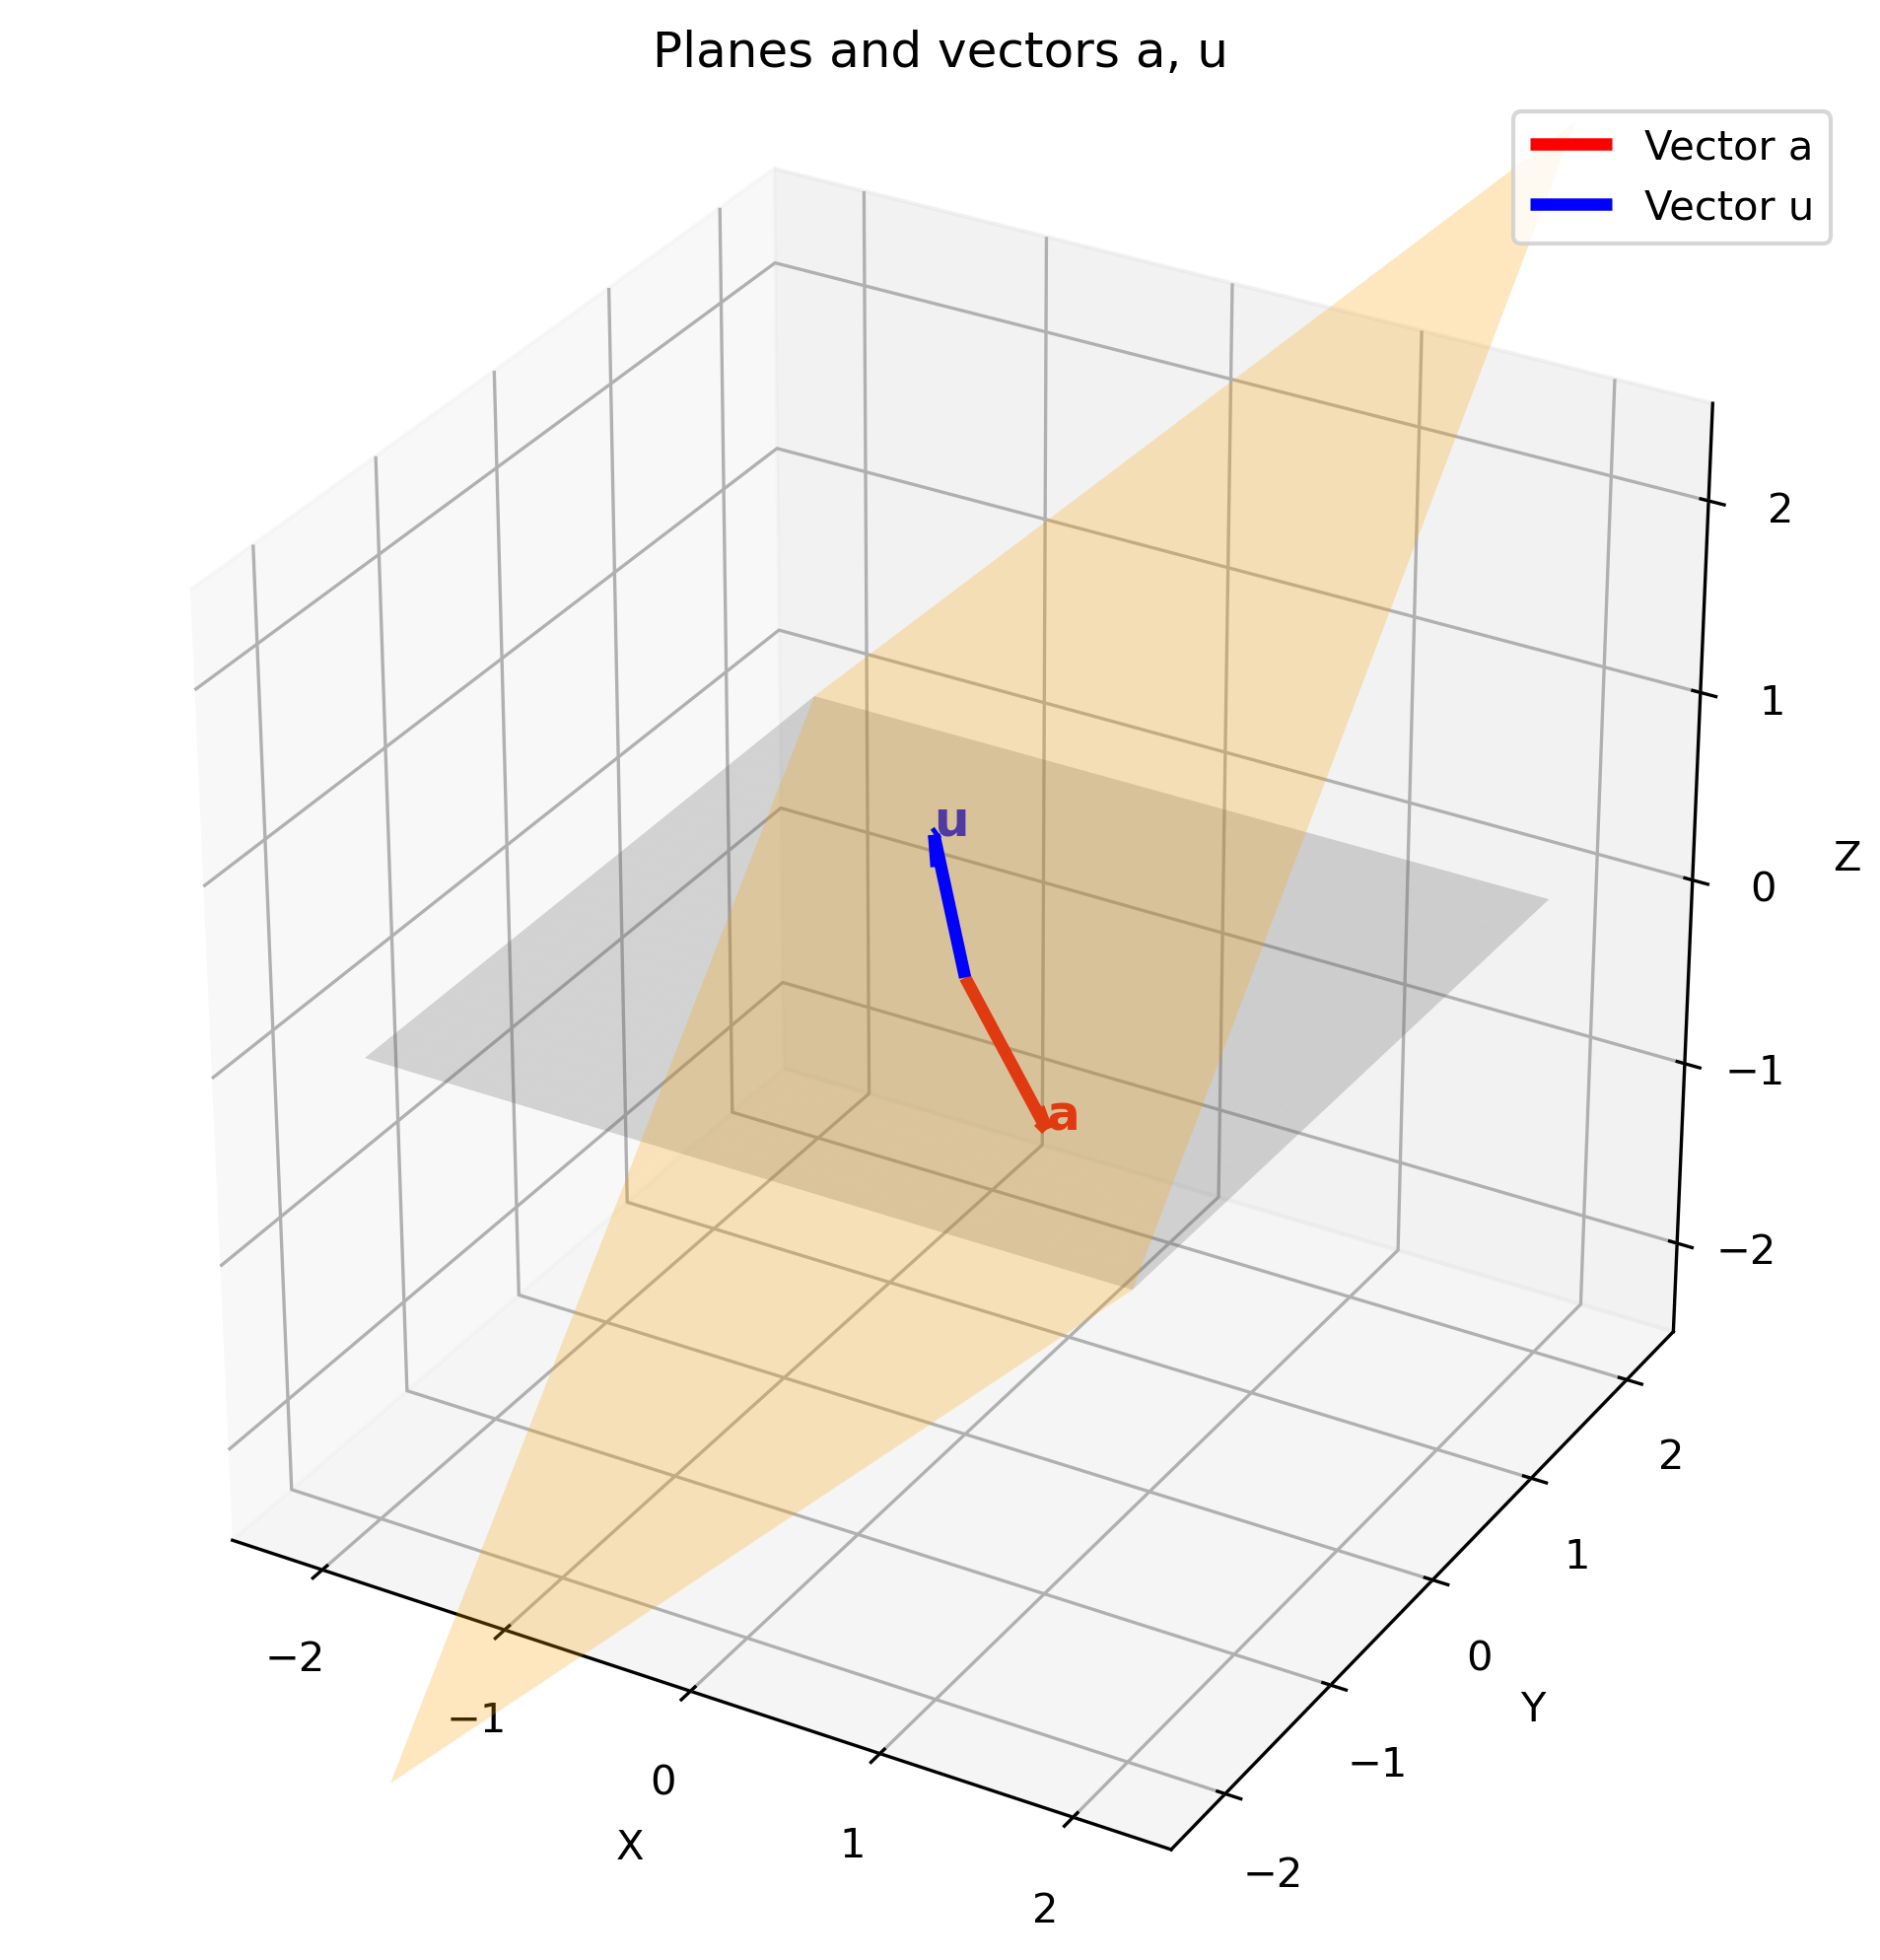
\includegraphics[width=\columnwidth, height=0.8\textheight, keepaspectratio]{figs/fig1.png}
    \label{fig:Beamer/figs/fig1.png}
\end{frame}


\end{document}